\documentclass[1p]{elsarticle_modified}
%\bibliographystyle{elsarticle-num}

%\usepackage[colorlinks]{hyperref}
%\usepackage{abbrmath_seonhwa} %\Abb, \Ascr, \Acal ,\Abf, \Afrak
\usepackage{amsfonts}
\usepackage{amssymb}
\usepackage{amsmath}
\usepackage{amsthm}
\usepackage{scalefnt}
\usepackage{amsbsy}
\usepackage{kotex}
\usepackage{caption}
\usepackage{subfig}
\usepackage{color}
\usepackage{graphicx}
\usepackage{xcolor} %% white, black, red, green, blue, cyan, magenta, yellow
\usepackage{float}
\usepackage{setspace}
\usepackage{hyperref}

\usepackage{tikz}
\usetikzlibrary{arrows}

\usepackage{multirow}
\usepackage{array} % fixed length table
\usepackage{hhline}

%%%%%%%%%%%%%%%%%%%%%
\makeatletter
\renewcommand*\env@matrix[1][\arraystretch]{%
	\edef\arraystretch{#1}%
	\hskip -\arraycolsep
	\let\@ifnextchar\new@ifnextchar
	\array{*\c@MaxMatrixCols c}}
\makeatother %https://tex.stackexchange.com/questions/14071/how-can-i-increase-the-line-spacing-in-a-matrix
%%%%%%%%%%%%%%%

\usepackage[normalem]{ulem}

\newcommand{\msout}[1]{\ifmmode\text{\sout{\ensuremath{#1}}}\else\sout{#1}\fi}
%SOURCE: \msout is \stkout macro in https://tex.stackexchange.com/questions/20609/strikeout-in-math-mode

\newcommand{\cancel}[1]{
	\ifmmode
	{\color{red}\msout{#1}}
	\else
	{\color{red}\sout{#1}}
	\fi
}

\newcommand{\add}[1]{
	{\color{blue}\uwave{#1}}
}

\newcommand{\replace}[2]{
	\ifmmode
	{\color{red}\msout{#1}}{\color{blue}\uwave{#2}}
	\else
	{\color{red}\sout{#1}}{\color{blue}\uwave{#2}}
	\fi
}

\newcommand{\Sol}{\mathcal{S}} %segment
\newcommand{\D}{D} %diagram
\newcommand{\A}{\mathcal{A}} %arc


%%%%%%%%%%%%%%%%%%%%%%%%%%%%%5 test

\def\sl{\operatorname{\textup{SL}}(2,\Cbb)}
\def\psl{\operatorname{\textup{PSL}}(2,\Cbb)}
\def\quan{\mkern 1mu \triangleright \mkern 1mu}

\theoremstyle{definition}
\newtheorem{thm}{Theorem}[section]
\newtheorem{prop}[thm]{Proposition}
\newtheorem{lem}[thm]{Lemma}
\newtheorem{ques}[thm]{Question}
\newtheorem{cor}[thm]{Corollary}
\newtheorem{defn}[thm]{Definition}
\newtheorem{exam}[thm]{Example}
\newtheorem{rmk}[thm]{Remark}
\newtheorem{alg}[thm]{Algorithm}

\newcommand{\I}{\sqrt{-1}}
\begin{document}

%\begin{frontmatter}
%
%\title{Boundary parabolic representations of knots up to 8 crossings}
%
%%% Group authors per affiliation:
%\author{Yunhi Cho} 
%\address{Department of Mathematics, University of Seoul, Seoul, Korea}
%\ead{yhcho@uos.ac.kr}
%
%
%\author{Seonhwa Kim} %\fnref{s_kim}}
%\address{Center for Geometry and Physics, Institute for Basic Science, Pohang, 37673, Korea}
%\ead{ryeona17@ibs.re.kr}
%
%\author{Hyuk Kim}
%\address{Department of Mathematical Sciences, Seoul National University, Seoul 08826, Korea}
%\ead{hyukkim@snu.ac.kr}
%
%\author{Seokbeom Yoon}
%\address{Department of Mathematical Sciences, Seoul National University, Seoul, 08826,  Korea}
%\ead{sbyoon15@snu.ac.kr}
%
%\begin{abstract}
%We find all boundary parabolic representation of knots up to 8 crossings.
%
%\end{abstract}
%\begin{keyword}
%    \MSC[2010] 57M25 
%\end{keyword}
%
%\end{frontmatter}

%\linenumbers
%\tableofcontents
%
\newcommand\colored[1]{\textcolor{white}{\rule[-0.35ex]{0.8em}{1.4ex}}\kern-0.8em\color{red} #1}%
%\newcommand\colored[1]{\textcolor{white}{ #1}\kern-2.17ex	\textcolor{white}{ #1}\kern-1.81ex	\textcolor{white}{ #1}\kern-2.15ex\color{red}#1	}

{\Large $\underline{11n_{146}~(K11n_{146})}$}

\setlength{\tabcolsep}{10pt}
\renewcommand{\arraystretch}{1.6}
\vspace{1cm}\begin{tabular}{m{100pt}>{\centering\arraybackslash}m{274pt}}
\multirow{5}{120pt}{
	\centering
	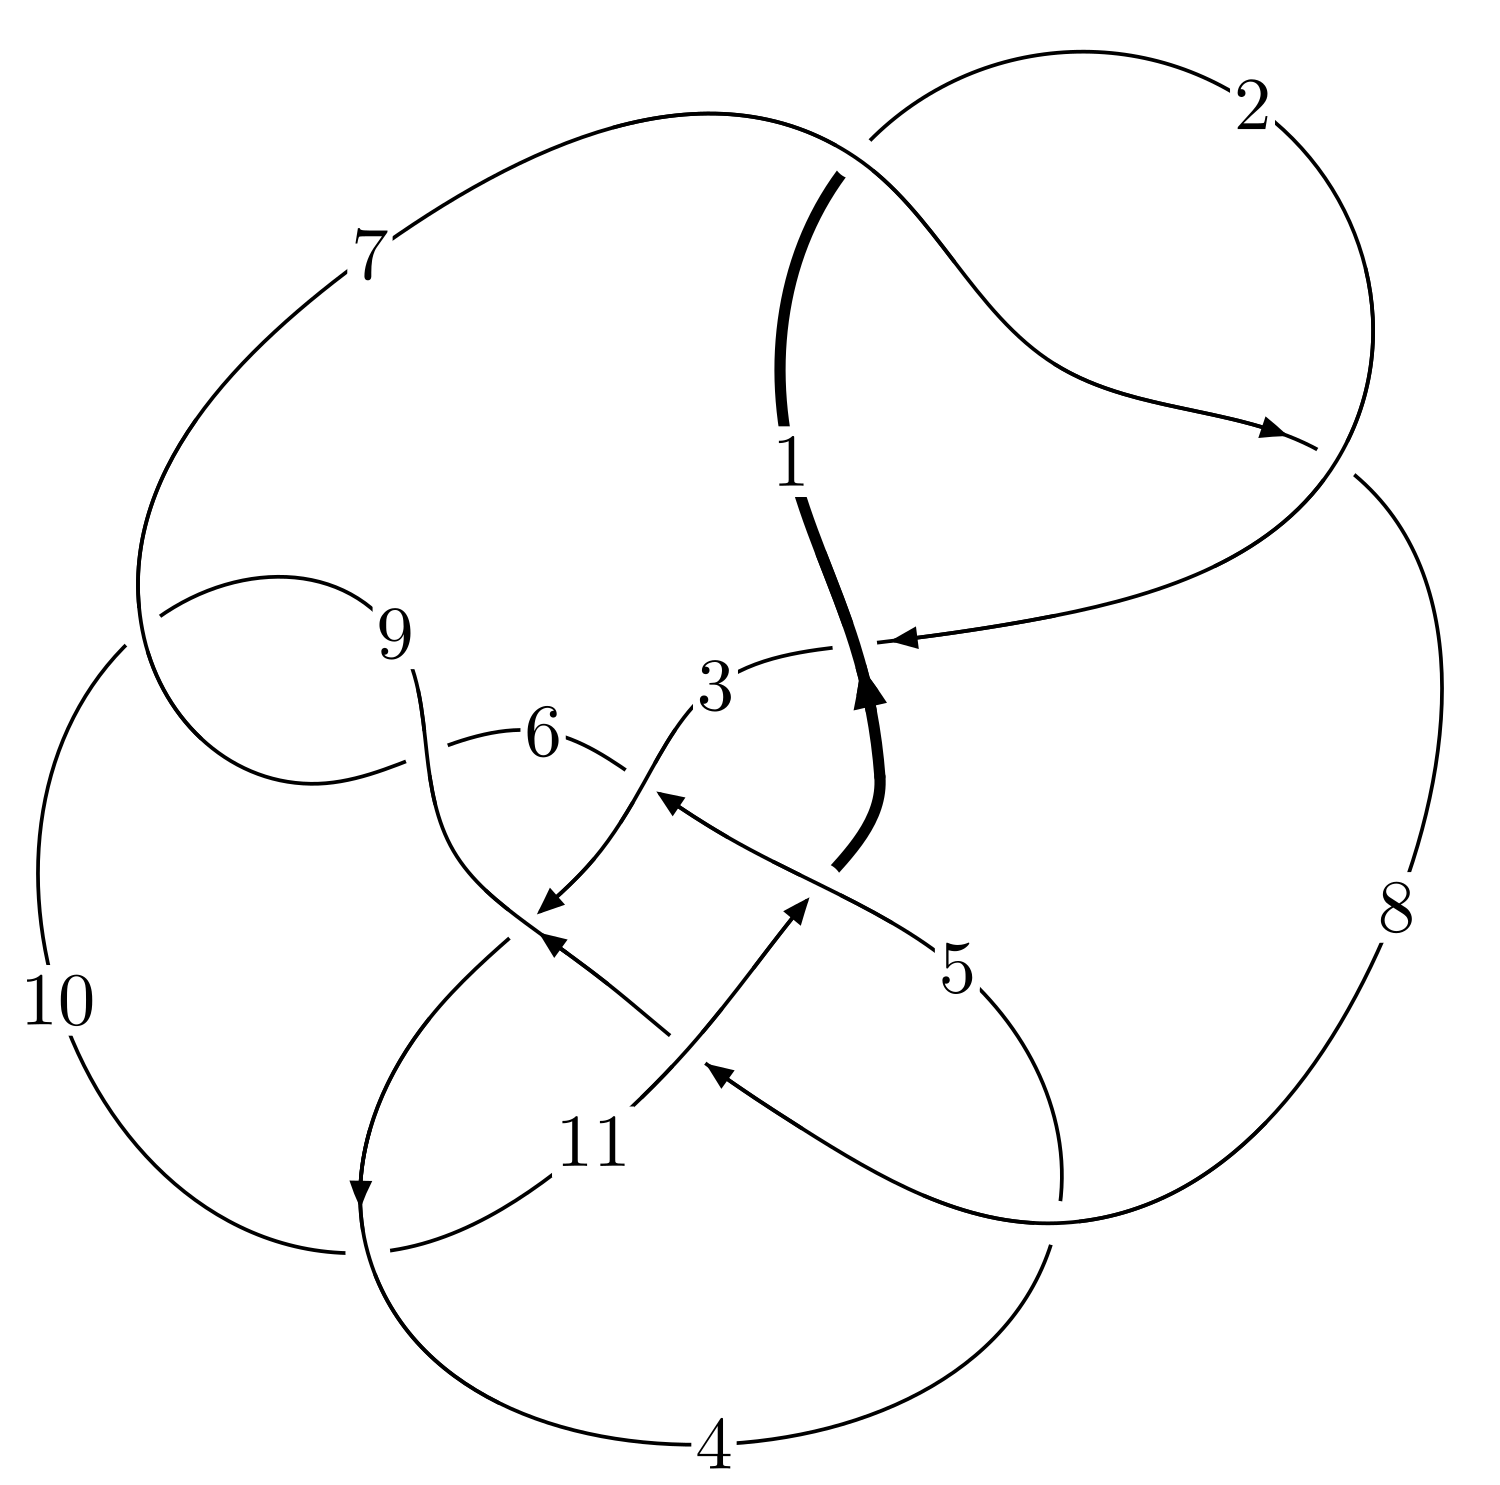
\includegraphics[width=112pt]{../../../GIT/diagram.site/Diagrams/png/762_11n_146.png}\\
\ \ \ A knot diagram\footnotemark}&
\allowdisplaybreaks
\textbf{Linearized knot diagam} \\
\cline{2-2}
 &
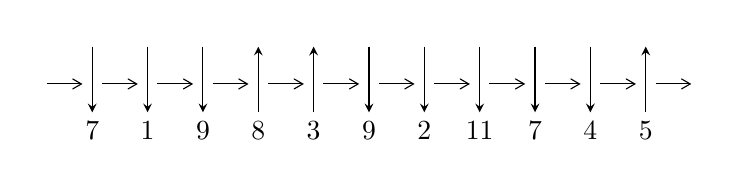
\begin{tikzpicture}[x=20pt, y=17pt]
	% nodes
	\node (C0) at (0, 0) {};
	\node (C1) at (1, 0) {};
	\node (C1U) at (1, +1) {};
	\node (C1D) at (1, -1) {7};

	\node (C2) at (2, 0) {};
	\node (C2U) at (2, +1) {};
	\node (C2D) at (2, -1) {1};

	\node (C3) at (3, 0) {};
	\node (C3U) at (3, +1) {};
	\node (C3D) at (3, -1) {9};

	\node (C4) at (4, 0) {};
	\node (C4U) at (4, +1) {};
	\node (C4D) at (4, -1) {8};

	\node (C5) at (5, 0) {};
	\node (C5U) at (5, +1) {};
	\node (C5D) at (5, -1) {3};

	\node (C6) at (6, 0) {};
	\node (C6U) at (6, +1) {};
	\node (C6D) at (6, -1) {9};

	\node (C7) at (7, 0) {};
	\node (C7U) at (7, +1) {};
	\node (C7D) at (7, -1) {2};

	\node (C8) at (8, 0) {};
	\node (C8U) at (8, +1) {};
	\node (C8D) at (8, -1) {11};

	\node (C9) at (9, 0) {};
	\node (C9U) at (9, +1) {};
	\node (C9D) at (9, -1) {7};

	\node (C10) at (10, 0) {};
	\node (C10U) at (10, +1) {};
	\node (C10D) at (10, -1) {4};

	\node (C11) at (11, 0) {};
	\node (C11U) at (11, +1) {};
	\node (C11D) at (11, -1) {5};
	\node (C12) at (12, 0) {};

	% arrows
	\draw[->,>={angle 60}]
	(C0) edge (C1) (C1) edge (C2) (C2) edge (C3) (C3) edge (C4) (C4) edge (C5) (C5) edge (C6) (C6) edge (C7) (C7) edge (C8) (C8) edge (C9) (C9) edge (C10) (C10) edge (C11) (C11) edge (C12) ;	\draw[->,>=stealth]
	(C1U) edge (C1D) (C2U) edge (C2D) (C3U) edge (C3D) (C4D) edge (C4U) (C5D) edge (C5U) (C6U) edge (C6D) (C7U) edge (C7D) (C8U) edge (C8D) (C9U) edge (C9D) (C10U) edge (C10D) (C11D) edge (C11U) ;
	\end{tikzpicture} \\
\hhline{~~} \\& 
\textbf{Solving Sequence} \\ \cline{2-2} 
 &
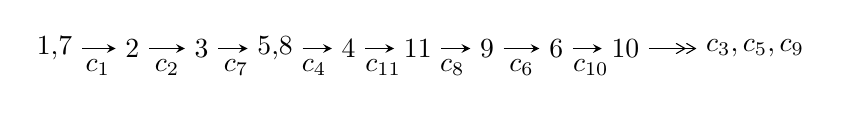
\begin{tikzpicture}[x=25pt, y=7pt]
	% node
	\node (A0) at (-1/8, 0) {1,7};
	\node (A1) at (1, 0) {2};
	\node (A2) at (2, 0) {3};
	\node (A3) at (49/16, 0) {5,8};
	\node (A4) at (33/8, 0) {4};
	\node (A5) at (41/8, 0) {11};
	\node (A6) at (49/8, 0) {9};
	\node (A7) at (57/8, 0) {6};
	\node (A8) at (65/8, 0) {10};
	\node (C1) at (1/2, -1) {$c_{1}$};
	\node (C2) at (3/2, -1) {$c_{2}$};
	\node (C3) at (5/2, -1) {$c_{7}$};
	\node (C4) at (29/8, -1) {$c_{4}$};
	\node (C5) at (37/8, -1) {$c_{11}$};
	\node (C6) at (45/8, -1) {$c_{8}$};
	\node (C7) at (53/8, -1) {$c_{6}$};
	\node (C8) at (61/8, -1) {$c_{10}$};
	\node (A9) at (10, 0) {$c_{3},c_{5},c_{9}$};

	% edge
	\draw[->,>=stealth]	
	(A0) edge (A1) (A1) edge (A2) (A2) edge (A3) (A3) edge (A4) (A4) edge (A5) (A5) edge (A6) (A6) edge (A7) (A7) edge (A8) ;
	\draw[->>,>={angle 60}]	
	(A8) edge (A9);
\end{tikzpicture} \\ 

\end{tabular} \\

\footnotetext{
The image of knot diagram is generated by the software ``\textbf{Draw programme}" developed by Andrew Bartholomew(\url{http://www.layer8.co.uk/maths/draw/index.htm\#Running-draw}), where we modified some parts for our purpose(\url{https://github.com/CATsTAILs/LinksPainter}).
}\phantom \\ \newline 
\centering \textbf{Ideals for irreducible components\footnotemark of $X_{\text{par}}$} 
 
\begin{align*}
I^u_{1}&=\langle 
9 u^{21}-99 u^{20}+\cdots+8 b+344,\;63 u^{21}-461 u^{20}+\cdots+16 a+368,\;u^{22}-9 u^{21}+\cdots+80 u-16\rangle \\
I^u_{2}&=\langle 
- u^{11}+4 u^9+u^8-7 u^7-2 u^6+8 u^5+4 u^4-6 u^3-5 u^2+b+2 u+3,\;u^{14}+2 u^{13}+\cdots+2 a-4,\\
\phantom{I^u_{2}}&\phantom{= \langle  }u^{15}-5 u^{13}- u^{12}+12 u^{11}+3 u^{10}-19 u^9-7 u^8+21 u^7+11 u^6-16 u^5-12 u^4+8 u^3+7 u^2-2 u-2\rangle \\
I^u_{3}&=\langle 
-34116957547 a^7 u^2+99566701011 a^6 u^2+\cdots+1815673106251 a+882543035301,\\
\phantom{I^u_{3}}&\phantom{= \langle  }3 a^7 u^2+7 a^6 u^2+\cdots-56 a+65,\;u^3+u^2-1\rangle \\
\\
\end{align*}
\raggedright * 3 irreducible components of $\dim_{\mathbb{C}}=0$, with total 61 representations.\\
\footnotetext{All coefficients of polynomials are rational numbers. But the coefficients are sometimes approximated in decimal forms when there is not enough margin.}
\newpage
\renewcommand{\arraystretch}{1}
\centering \section*{I. $I^u_{1}= \langle 9 u^{21}-99 u^{20}+\cdots+8 b+344,\;63 u^{21}-461 u^{20}+\cdots+16 a+368,\;u^{22}-9 u^{21}+\cdots+80 u-16 \rangle$}
\flushleft \textbf{(i) Arc colorings}\\
\begin{tabular}{m{7pt} m{180pt} m{7pt} m{180pt} }
\flushright $a_{1}=$&$\begin{pmatrix}1\\0\end{pmatrix}$ \\
\flushright $a_{7}=$&$\begin{pmatrix}0\\u\end{pmatrix}$ \\
\flushright $a_{2}=$&$\begin{pmatrix}1\\u^2\end{pmatrix}$ \\
\flushright $a_{3}=$&$\begin{pmatrix}- u^2+1\\u^2\end{pmatrix}$ \\
\flushright $a_{5}=$&$\begin{pmatrix}-\frac{63}{16} u^{21}+\frac{461}{16} u^{20}+\cdots+\frac{229}{2} u-23\\-\frac{9}{8} u^{21}+\frac{99}{8} u^{20}+\cdots+175 u-43\end{pmatrix}$ \\
\flushright $a_{8}=$&$\begin{pmatrix}- u\\- u^3+u\end{pmatrix}$ \\
\flushright $a_{4}=$&$\begin{pmatrix}-\frac{27}{16} u^{21}+\frac{241}{16} u^{20}+\cdots+\frac{323}{2} u-41\\\frac{53}{8} u^{21}-\frac{423}{8} u^{20}+\cdots-356 u+79\end{pmatrix}$ \\
\flushright $a_{11}=$&$\begin{pmatrix}9 u^{21}-\frac{557}{8} u^{20}+\cdots-\frac{1413}{4} u+\frac{135}{2}\\-\frac{7}{8} u^{21}+\frac{31}{8} u^{20}+\cdots-\frac{225}{2} u+38\end{pmatrix}$ \\
\flushright $a_{9}=$&$\begin{pmatrix}-0.0625000 u^{21}+2.06250 u^{20}+\cdots+41.2500 u-11.5000\\\frac{19}{4} u^{21}-\frac{79}{2} u^{20}+\cdots-\frac{623}{2} u+75\end{pmatrix}$ \\
\flushright $a_{6}=$&$\begin{pmatrix}\frac{27}{16} u^{21}-\frac{241}{16} u^{20}+\cdots-\frac{323}{2} u+40\\-\frac{53}{8} u^{21}+\frac{423}{8} u^{20}+\cdots+357 u-79\end{pmatrix}$ \\
\flushright $a_{10}=$&$\begin{pmatrix}-0.0625000 u^{21}+2.06250 u^{20}+\cdots+41.2500 u-11.5000\\\frac{17}{2} u^{21}-\frac{271}{4} u^{20}+\cdots-\frac{865}{2} u+99\end{pmatrix}$\\ \flushright $a_{10}=$&$\begin{pmatrix}-0.0625000 u^{21}+2.06250 u^{20}+\cdots+41.2500 u-11.5000\\\frac{17}{2} u^{21}-\frac{271}{4} u^{20}+\cdots-\frac{865}{2} u+99\end{pmatrix}$\\&\end{tabular}
\flushleft \textbf{(ii) Obstruction class $= -1$}\\~\\
\flushleft \textbf{(iii) Cusp Shapes $= -\frac{39}{2} u^{21}+\frac{301}{2} u^{20}+\cdots+914 u-202$}\\~\\
\newpage\renewcommand{\arraystretch}{1}
\flushleft \textbf{(iv) u-Polynomials at the component}\newline \\
\begin{tabular}{m{50pt}|m{274pt}}
Crossings & \hspace{64pt}u-Polynomials at each crossing \\
\hline $$\begin{aligned}c_{1},c_{7}\end{aligned}$$&$\begin{aligned}
&u^{22}-9 u^{21}+\cdots+80 u-16
\end{aligned}$\\
\hline $$\begin{aligned}c_{2}\end{aligned}$$&$\begin{aligned}
&u^{22}+11 u^{21}+\cdots+1408 u+256
\end{aligned}$\\
\hline $$\begin{aligned}c_{3},c_{6},c_{9}\end{aligned}$$&$\begin{aligned}
&u^{22}+18 u^{20}+\cdots-3 u-1
\end{aligned}$\\
\hline $$\begin{aligned}c_{4},c_{11}\end{aligned}$$&$\begin{aligned}
&u^{22}-6 u^{20}+\cdots+4 u-1
\end{aligned}$\\
\hline $$\begin{aligned}c_{5}\end{aligned}$$&$\begin{aligned}
&u^{22}+12 u^{21}+\cdots+672 u+64
\end{aligned}$\\
\hline $$\begin{aligned}c_{8}\end{aligned}$$&$\begin{aligned}
&u^{22}-12 u^{21}+\cdots-64 u+8
\end{aligned}$\\
\hline $$\begin{aligned}c_{10}\end{aligned}$$&$\begin{aligned}
&u^{22}+u^{21}+\cdots-2 u^2-10
\end{aligned}$\\
\hline
\end{tabular}\\~\\
\newpage\renewcommand{\arraystretch}{1}
\flushleft \textbf{(v) Riley Polynomials at the component}\newline \\
\begin{tabular}{m{50pt}|m{274pt}}
Crossings & \hspace{64pt}Riley Polynomials at each crossing \\
\hline $$\begin{aligned}c_{1},c_{7}\end{aligned}$$&$\begin{aligned}
&y^{22}-11 y^{21}+\cdots-1408 y+256
\end{aligned}$\\
\hline $$\begin{aligned}c_{2}\end{aligned}$$&$\begin{aligned}
&y^{22}+y^{21}+\cdots-663552 y+65536
\end{aligned}$\\
\hline $$\begin{aligned}c_{3},c_{6},c_{9}\end{aligned}$$&$\begin{aligned}
&y^{22}+36 y^{21}+\cdots+9 y+1
\end{aligned}$\\
\hline $$\begin{aligned}c_{4},c_{11}\end{aligned}$$&$\begin{aligned}
&y^{22}-12 y^{21}+\cdots-66 y+1
\end{aligned}$\\
\hline $$\begin{aligned}c_{5}\end{aligned}$$&$\begin{aligned}
&y^{22}-26 y^{21}+\cdots-273920 y+4096
\end{aligned}$\\
\hline $$\begin{aligned}c_{8}\end{aligned}$$&$\begin{aligned}
&y^{22}-2 y^{21}+\cdots+224 y+64
\end{aligned}$\\
\hline $$\begin{aligned}c_{10}\end{aligned}$$&$\begin{aligned}
&y^{22}+19 y^{21}+\cdots+40 y+100
\end{aligned}$\\
\hline
\end{tabular}\\~\\
\newpage\flushleft \textbf{(vi) Complex Volumes and Cusp Shapes}
$$\begin{array}{c|c|c}  
\text{Solutions to }I^u_{1}& \I (\text{vol} + \sqrt{-1}CS) & \text{Cusp shape}\\
 \hline 
\begin{aligned}
u &= -1.066710 + 0.226222 I \\
a &= -0.351526 + 0.307053 I \\
b &= -0.539318 + 0.910382 I\end{aligned}
 & -2.44040 + 0.11720 I & -7.20404 - 1.75445 I \\ \hline\begin{aligned}
u &= -1.066710 - 0.226222 I \\
a &= -0.351526 - 0.307053 I \\
b &= -0.539318 - 0.910382 I\end{aligned}
 & -2.44040 - 0.11720 I & -7.20404 + 1.75445 I \\ \hline\begin{aligned}
u &= \phantom{-}1.039800 + 0.529986 I \\
a &= \phantom{-}0.729503 + 1.140060 I \\
b &= -0.827030 + 0.144364 I\end{aligned}
 & \phantom{-}0.80566 - 4.34766 I & -4.70703 + 6.76579 I \\ \hline\begin{aligned}
u &= \phantom{-}1.039800 - 0.529986 I \\
a &= \phantom{-}0.729503 - 1.140060 I \\
b &= -0.827030 - 0.144364 I\end{aligned}
 & \phantom{-}0.80566 + 4.34766 I & -4.70703 - 6.76579 I \\ \hline\begin{aligned}
u &= \phantom{-}0.392350 + 0.705715 I \\
a &= -1.47104 - 0.61591 I \\
b &= \phantom{-}0.989758 + 0.677091 I\end{aligned}
 & \phantom{-}1.86600 + 2.08328 I & \phantom{-}1.28577 - 1.87912 I \\ \hline\begin{aligned}
u &= \phantom{-}0.392350 - 0.705715 I \\
a &= -1.47104 + 0.61591 I \\
b &= \phantom{-}0.989758 - 0.677091 I\end{aligned}
 & \phantom{-}1.86600 - 2.08328 I & \phantom{-}1.28577 + 1.87912 I \\ \hline\begin{aligned}
u &= \phantom{-}0.583477 + 1.050930 I \\
a &= \phantom{-}0.954459 + 0.738545 I \\
b &= -1.41570 - 0.82771 I\end{aligned}
 & \phantom{-}11.22610 + 7.92016 I & -1.17318 - 3.44504 I \\ \hline\begin{aligned}
u &= \phantom{-}0.583477 - 1.050930 I \\
a &= \phantom{-}0.954459 - 0.738545 I \\
b &= -1.41570 + 0.82771 I\end{aligned}
 & \phantom{-}11.22610 - 7.92016 I & -1.17318 + 3.44504 I \\ \hline\begin{aligned}
u &= \phantom{-}0.498409 + 0.620816 I \\
a &= -1.379510 + 0.247291 I \\
b &= \phantom{-}0.877040 - 0.154406 I\end{aligned}
 & \phantom{-}2.40742 - 0.20200 I & -0.358944 + 0.576250 I \\ \hline\begin{aligned}
u &= \phantom{-}0.498409 - 0.620816 I \\
a &= -1.379510 - 0.247291 I \\
b &= \phantom{-}0.877040 + 0.154406 I\end{aligned}
 & \phantom{-}2.40742 + 0.20200 I & -0.358944 - 0.576250 I\\
 \hline 
 \end{array}$$\newpage$$\begin{array}{c|c|c}  
\text{Solutions to }I^u_{1}& \I (\text{vol} + \sqrt{-1}CS) & \text{Cusp shape}\\
 \hline 
\begin{aligned}
u &= \phantom{-}1.091100 + 0.568772 I \\
a &= \phantom{-}1.66508 + 1.05767 I \\
b &= -1.084320 + 0.882593 I\end{aligned}
 & -0.17078 - 6.97976 I & -0.36212 + 5.29220 I \\ \hline\begin{aligned}
u &= \phantom{-}1.091100 - 0.568772 I \\
a &= \phantom{-}1.66508 - 1.05767 I \\
b &= -1.084320 - 0.882593 I\end{aligned}
 & -0.17078 + 6.97976 I & -0.36212 - 5.29220 I \\ \hline\begin{aligned}
u &= \phantom{-}0.520231 + 1.151080 I \\
a &= \phantom{-}0.694248 + 0.193737 I \\
b &= -1.102170 - 0.272719 I\end{aligned}
 & \phantom{-}10.39030 - 0.61941 I & \phantom{-}1.005762 + 0.209971 I \\ \hline\begin{aligned}
u &= \phantom{-}0.520231 - 1.151080 I \\
a &= \phantom{-}0.694248 - 0.193737 I \\
b &= -1.102170 + 0.272719 I\end{aligned}
 & \phantom{-}10.39030 + 0.61941 I & \phantom{-}1.005762 - 0.209971 I \\ \hline\begin{aligned}
u &= \phantom{-}1.154680 + 0.769733 I \\
a &= -1.41430 - 0.79322 I \\
b &= \phantom{-}1.38480 - 1.09712 I\end{aligned}
 & \phantom{-}9.4240 - 14.4970 I & -3.20540 + 7.40924 I \\ \hline\begin{aligned}
u &= \phantom{-}1.154680 - 0.769733 I \\
a &= -1.41430 + 0.79322 I \\
b &= \phantom{-}1.38480 + 1.09712 I\end{aligned}
 & \phantom{-}9.4240 + 14.4970 I & -3.20540 - 7.40924 I \\ \hline\begin{aligned}
u &= \phantom{-}1.21138 + 0.80873 I \\
a &= -0.770380 - 0.556560 I \\
b &= \phantom{-}0.946982 - 0.664925 I\end{aligned}
 & \phantom{-}8.24676 - 6.35399 I & -2.34309 + 5.14871 I \\ \hline\begin{aligned}
u &= \phantom{-}1.21138 - 0.80873 I \\
a &= -0.770380 + 0.556560 I \\
b &= \phantom{-}0.946982 + 0.664925 I\end{aligned}
 & \phantom{-}8.24676 + 6.35399 I & -2.34309 - 5.14871 I \\ \hline\begin{aligned}
u &= -1.46566 + 0.12857 I \\
a &= \phantom{-}0.213752 + 0.149488 I \\
b &= \phantom{-}0.844485 + 0.429706 I\end{aligned}
 & \phantom{-}2.91041 + 4.96923 I & -3.04819 - 6.01952 I \\ \hline\begin{aligned}
u &= -1.46566 - 0.12857 I \\
a &= \phantom{-}0.213752 - 0.149488 I \\
b &= \phantom{-}0.844485 - 0.429706 I\end{aligned}
 & \phantom{-}2.91041 - 4.96923 I & -3.04819 + 6.01952 I\\
 \hline 
 \end{array}$$\newpage$$\begin{array}{c|c|c}  
\text{Solutions to }I^u_{1}& \I (\text{vol} + \sqrt{-1}CS) & \text{Cusp shape}\\
 \hline 
\begin{aligned}
u &= -0.492053\phantom{ +0.000000I} \\
a &= -0.403784\phantom{ +0.000000I} \\
b &= -0.296446\phantom{ +0.000000I}\end{aligned}
 & -0.825428\phantom{ +0.000000I} & -11.7690\phantom{ +0.000000I} \\ \hline\begin{aligned}
u &= \phantom{-}1.57389\phantom{ +0.000000I} \\
a &= \phantom{-}0.163193\phantom{ +0.000000I} \\
b &= \phantom{-}0.147402\phantom{ +0.000000I}\end{aligned}
 & -7.90371\phantom{ +0.000000I} & -59.0100\phantom{ +0.000000I}\\
 \hline 
 \end{array}$$\newpage\newpage\renewcommand{\arraystretch}{1}
\centering \section*{II. $I^u_{2}= \langle - u^{11}+4 u^9+\cdots+b+3,\;u^{14}+2 u^{13}+\cdots+2 a-4,\;u^{15}-5 u^{13}+\cdots-2 u-2 \rangle$}
\flushleft \textbf{(i) Arc colorings}\\
\begin{tabular}{m{7pt} m{180pt} m{7pt} m{180pt} }
\flushright $a_{1}=$&$\begin{pmatrix}1\\0\end{pmatrix}$ \\
\flushright $a_{7}=$&$\begin{pmatrix}0\\u\end{pmatrix}$ \\
\flushright $a_{2}=$&$\begin{pmatrix}1\\u^2\end{pmatrix}$ \\
\flushright $a_{3}=$&$\begin{pmatrix}- u^2+1\\u^2\end{pmatrix}$ \\
\flushright $a_{5}=$&$\begin{pmatrix}-\frac{1}{2} u^{14}- u^{13}+\cdots-\frac{13}{2} u+2\\u^{11}-4 u^9- u^8+7 u^7+2 u^6-8 u^5-4 u^4+6 u^3+5 u^2-2 u-3\end{pmatrix}$ \\
\flushright $a_{8}=$&$\begin{pmatrix}- u\\- u^3+u\end{pmatrix}$ \\
\flushright $a_{4}=$&$\begin{pmatrix}-\frac{1}{2} u^{14}- u^{13}+\cdots-\frac{7}{2} u+2\\- u^{14}+5 u^{12}+\cdots-5 u-3\end{pmatrix}$ \\
\flushright $a_{11}=$&$\begin{pmatrix}\frac{5}{2} u^{14}-\frac{23}{2} u^{12}+\cdots+\frac{9}{2} u-5\\u^{14}+2 u^{13}+\cdots+4 u+5\end{pmatrix}$ \\
\flushright $a_{9}=$&$\begin{pmatrix}-\frac{3}{2} u^{14}+u^{13}+\cdots-\frac{7}{2} u+2\\4 u^{14}+3 u^{13}+\cdots+12 u+5\end{pmatrix}$ \\
\flushright $a_{6}=$&$\begin{pmatrix}-\frac{1}{2} u^{14}- u^{13}+\cdots-\frac{7}{2} u+1\\- u^{14}+5 u^{12}+\cdots-4 u-3\end{pmatrix}$ \\
\flushright $a_{10}=$&$\begin{pmatrix}-\frac{3}{2} u^{14}+u^{13}+\cdots-\frac{7}{2} u+2\\4 u^{14}+4 u^{13}+\cdots+11 u+7\end{pmatrix}$\\ \flushright $a_{10}=$&$\begin{pmatrix}-\frac{3}{2} u^{14}+u^{13}+\cdots-\frac{7}{2} u+2\\4 u^{14}+4 u^{13}+\cdots+11 u+7\end{pmatrix}$\\&\end{tabular}
\flushleft \textbf{(ii) Obstruction class $= 1$}\\~\\
\flushleft \textbf{(iii) Cusp Shapes $= -8 u^{14}-11 u^{13}+37 u^{12}+56 u^{11}-69 u^{10}-119 u^9+89 u^8+182 u^7-56 u^6-195 u^5-6 u^4+135 u^3+41 u^2-48 u-22$}\\~\\
\newpage\renewcommand{\arraystretch}{1}
\flushleft \textbf{(iv) u-Polynomials at the component}\newline \\
\begin{tabular}{m{50pt}|m{274pt}}
Crossings & \hspace{64pt}u-Polynomials at each crossing \\
\hline $$\begin{aligned}c_{1}\end{aligned}$$&$\begin{aligned}
&u^{15}-5 u^{13}+\cdots-2 u-2
\end{aligned}$\\
\hline $$\begin{aligned}c_{2}\end{aligned}$$&$\begin{aligned}
&u^{15}+10 u^{14}+\cdots+32 u+4
\end{aligned}$\\
\hline $$\begin{aligned}c_{3},c_{9}\end{aligned}$$&$\begin{aligned}
&u^{15}+4 u^{13}+\cdots+u-1
\end{aligned}$\\
\hline $$\begin{aligned}c_{4},c_{11}\end{aligned}$$&$\begin{aligned}
&u^{15}+2 u^{13}+\cdots+4 u-1
\end{aligned}$\\
\hline $$\begin{aligned}c_{5}\end{aligned}$$&$\begin{aligned}
&u^{15}-11 u^{14}+\cdots+73 u-25
\end{aligned}$\\
\hline $$\begin{aligned}c_{6}\end{aligned}$$&$\begin{aligned}
&u^{15}+4 u^{13}+\cdots+u+1
\end{aligned}$\\
\hline $$\begin{aligned}c_{7}\end{aligned}$$&$\begin{aligned}
&u^{15}-5 u^{13}+\cdots-2 u+2
\end{aligned}$\\
\hline $$\begin{aligned}c_{8}\end{aligned}$$&$\begin{aligned}
&u^{15}-7 u^{14}+\cdots+3 u^2-1
\end{aligned}$\\
\hline $$\begin{aligned}c_{10}\end{aligned}$$&$\begin{aligned}
&u^{15}+u^{14}+\cdots+2 u+2
\end{aligned}$\\
\hline
\end{tabular}\\~\\
\newpage\renewcommand{\arraystretch}{1}
\flushleft \textbf{(v) Riley Polynomials at the component}\newline \\
\begin{tabular}{m{50pt}|m{274pt}}
Crossings & \hspace{64pt}Riley Polynomials at each crossing \\
\hline $$\begin{aligned}c_{1},c_{7}\end{aligned}$$&$\begin{aligned}
&y^{15}-10 y^{14}+\cdots+32 y-4
\end{aligned}$\\
\hline $$\begin{aligned}c_{2}\end{aligned}$$&$\begin{aligned}
&y^{15}-2 y^{14}+\cdots-8 y-16
\end{aligned}$\\
\hline $$\begin{aligned}c_{3},c_{6},c_{9}\end{aligned}$$&$\begin{aligned}
&y^{15}+8 y^{14}+\cdots+11 y-1
\end{aligned}$\\
\hline $$\begin{aligned}c_{4},c_{11}\end{aligned}$$&$\begin{aligned}
&y^{15}+4 y^{14}+\cdots+14 y-1
\end{aligned}$\\
\hline $$\begin{aligned}c_{5}\end{aligned}$$&$\begin{aligned}
&y^{15}-19 y^{14}+\cdots+4329 y-625
\end{aligned}$\\
\hline $$\begin{aligned}c_{8}\end{aligned}$$&$\begin{aligned}
&y^{15}-3 y^{14}+\cdots+6 y-1
\end{aligned}$\\
\hline $$\begin{aligned}c_{10}\end{aligned}$$&$\begin{aligned}
&y^{15}+7 y^{14}+\cdots+39 y^2-4
\end{aligned}$\\
\hline
\end{tabular}\\~\\
\newpage\flushleft \textbf{(vi) Complex Volumes and Cusp Shapes}
$$\begin{array}{c|c|c}  
\text{Solutions to }I^u_{2}& \I (\text{vol} + \sqrt{-1}CS) & \text{Cusp shape}\\
 \hline 
\begin{aligned}
u &= \phantom{-}0.945062 + 0.354082 I \\
a &= \phantom{-}0.565133 + 0.388167 I \\
b &= \phantom{-}0.570749 + 1.243190 I\end{aligned}
 & -3.02280 + 1.54146 I & -6.80860 + 0.33073 I \\ \hline\begin{aligned}
u &= \phantom{-}0.945062 - 0.354082 I \\
a &= \phantom{-}0.565133 - 0.388167 I \\
b &= \phantom{-}0.570749 - 1.243190 I\end{aligned}
 & -3.02280 - 1.54146 I & -6.80860 - 0.33073 I \\ \hline\begin{aligned}
u &= -0.573037 + 0.772166 I \\
a &= \phantom{-}0.944181 - 0.805222 I \\
b &= -0.884792 + 0.570619 I\end{aligned}
 & \phantom{-}0.37010 - 2.03676 I & -5.30954 + 3.27219 I \\ \hline\begin{aligned}
u &= -0.573037 - 0.772166 I \\
a &= \phantom{-}0.944181 + 0.805222 I \\
b &= -0.884792 - 0.570619 I\end{aligned}
 & \phantom{-}0.37010 + 2.03676 I & -5.30954 - 3.27219 I \\ \hline\begin{aligned}
u &= \phantom{-}0.869875 + 0.302392 I \\
a &= \phantom{-}0.175063 + 0.651509 I \\
b &= -0.271019 + 1.145180 I\end{aligned}
 & -2.66889 - 4.30403 I & -6.64337 + 8.95164 I \\ \hline\begin{aligned}
u &= \phantom{-}0.869875 - 0.302392 I \\
a &= \phantom{-}0.175063 - 0.651509 I \\
b &= -0.271019 - 1.145180 I\end{aligned}
 & -2.66889 + 4.30403 I & -6.64337 - 8.95164 I \\ \hline\begin{aligned}
u &= \phantom{-}0.867167 + 0.769940 I \\
a &= -0.507277 - 0.120829 I \\
b &= -0.266261 - 1.191970 I\end{aligned}
 & \phantom{-}7.81854 - 2.90716 I & -1.49116 + 2.36324 I \\ \hline\begin{aligned}
u &= \phantom{-}0.867167 - 0.769940 I \\
a &= -0.507277 + 0.120829 I \\
b &= -0.266261 + 1.191970 I\end{aligned}
 & \phantom{-}7.81854 + 2.90716 I & -1.49116 - 2.36324 I \\ \hline\begin{aligned}
u &= -1.042710 + 0.599702 I \\
a &= -1.70977 + 0.73314 I \\
b &= \phantom{-}1.015990 + 0.881908 I\end{aligned}
 & -1.08562 + 7.20573 I & -9.25026 - 7.69565 I \\ \hline\begin{aligned}
u &= -1.042710 - 0.599702 I \\
a &= -1.70977 - 0.73314 I \\
b &= \phantom{-}1.015990 - 0.881908 I\end{aligned}
 & -1.08562 - 7.20573 I & -9.25026 + 7.69565 I\\
 \hline 
 \end{array}$$\newpage$$\begin{array}{c|c|c}  
\text{Solutions to }I^u_{2}& \I (\text{vol} + \sqrt{-1}CS) & \text{Cusp shape}\\
 \hline 
\begin{aligned}
u &= -1.173890 + 0.354715 I \\
a &= \phantom{-}0.415207 + 1.215040 I \\
b &= \phantom{-}0.613391 - 0.103361 I\end{aligned}
 & \phantom{-}2.75922 + 3.34728 I & -2.20513 - 3.30365 I \\ \hline\begin{aligned}
u &= -1.173890 - 0.354715 I \\
a &= \phantom{-}0.415207 - 1.215040 I \\
b &= \phantom{-}0.613391 + 0.103361 I\end{aligned}
 & \phantom{-}2.75922 - 3.34728 I & -2.20513 + 3.30365 I \\ \hline\begin{aligned}
u &= -0.691226 + 0.240625 I \\
a &= \phantom{-}3.57976 + 0.40015 I \\
b &= -0.934484 - 0.438009 I\end{aligned}
 & \phantom{-}4.67692 - 0.80845 I & \phantom{-}3.56798 - 2.11727 I \\ \hline\begin{aligned}
u &= -0.691226 - 0.240625 I \\
a &= \phantom{-}3.57976 - 0.40015 I \\
b &= -0.934484 + 0.438009 I\end{aligned}
 & \phantom{-}4.67692 + 0.80845 I & \phantom{-}3.56798 + 2.11727 I \\ \hline\begin{aligned}
u &= \phantom{-}1.59751\phantom{ +0.000000I} \\
a &= \phantom{-}0.0753958\phantom{ +0.000000I} \\
b &= \phantom{-}0.312857\phantom{ +0.000000I}\end{aligned}
 & -7.82532\phantom{ +0.000000I} & \phantom{-}43.2800\phantom{ +0.000000I}\\
 \hline 
 \end{array}$$\newpage\newpage\renewcommand{\arraystretch}{1}
\centering \section*{III. $I^u_{3}= \langle -3.41\times10^{10} a^{7} u^{2}+9.96\times10^{10} a^{6} u^{2}+\cdots+1.82\times10^{12} a+8.83\times10^{11},\;3 a^7 u^2+7 a^6 u^2+\cdots-56 a+65,\;u^3+u^2-1 \rangle$}
\flushleft \textbf{(i) Arc colorings}\\
\begin{tabular}{m{7pt} m{180pt} m{7pt} m{180pt} }
\flushright $a_{1}=$&$\begin{pmatrix}1\\0\end{pmatrix}$ \\
\flushright $a_{7}=$&$\begin{pmatrix}0\\u\end{pmatrix}$ \\
\flushright $a_{2}=$&$\begin{pmatrix}1\\u^2\end{pmatrix}$ \\
\flushright $a_{3}=$&$\begin{pmatrix}- u^2+1\\u^2\end{pmatrix}$ \\
\flushright $a_{5}=$&$\begin{pmatrix}a\\0.00955622 a^{7} u^{2}-0.0278888 a^{6} u^{2}+\cdots-0.508573 a-0.247202\end{pmatrix}$ \\
\flushright $a_{8}=$&$\begin{pmatrix}- u\\u^2+u-1\end{pmatrix}$ \\
\flushright $a_{4}=$&$\begin{pmatrix}-0.0206730 a^{7} u^{2}+0.00671494 a^{6} u^{2}+\cdots-0.167214 a+0.361442\\0.0365923 a^{7} u^{2}-0.106197 a^{6} u^{2}+\cdots+0.254915 a-0.349774\end{pmatrix}$ \\
\flushright $a_{11}=$&$\begin{pmatrix}-0.0136970 a^{7} u^{2}+0.167653 a^{6} u^{2}+\cdots-0.128713 a+0.671444\\0.0545800 a^{7} u^{2}-0.0709107 a^{6} u^{2}+\cdots-0.318374 a-0.618795\end{pmatrix}$ \\
\flushright $a_{9}=$&$\begin{pmatrix}-0.0337296 a^{7} u^{2}-0.0293879 a^{6} u^{2}+\cdots+0.243004 a+1.20707\\-0.0280221 a^{7} u^{2}+0.0695256 a^{6} u^{2}+\cdots+0.701359 a-0.906712\end{pmatrix}$ \\
\flushright $a_{6}=$&$\begin{pmatrix}-0.0381529 a^{7} u^{2}+0.0571347 a^{6} u^{2}+\cdots+0.560725 a+0.216812\\0.0365923 a^{7} u^{2}-0.106197 a^{6} u^{2}+\cdots-0.745085 a-0.349774\end{pmatrix}$ \\
\flushright $a_{10}=$&$\begin{pmatrix}-0.0337296 a^{7} u^{2}-0.0293879 a^{6} u^{2}+\cdots+0.243004 a+1.20707\\-0.0419144 a^{7} u^{2}+0.0898677 a^{6} u^{2}+\cdots+1.22012 a-0.592528\end{pmatrix}$\\ \flushright $a_{10}=$&$\begin{pmatrix}-0.0337296 a^{7} u^{2}-0.0293879 a^{6} u^{2}+\cdots+0.243004 a+1.20707\\-0.0419144 a^{7} u^{2}+0.0898677 a^{6} u^{2}+\cdots+1.22012 a-0.592528\end{pmatrix}$\\&\end{tabular}
\flushleft \textbf{(ii) Obstruction class $= -1$}\\~\\
\flushleft \textbf{(iii) Cusp Shapes $= -\frac{1164454014992}{3570132856135} a^7 u^2+\frac{1180088464472}{3570132856135} a^6 u^2+\cdots-\frac{4943997575288}{3570132856135} a-\frac{7861314901686}{3570132856135}$}\\~\\
\newpage\renewcommand{\arraystretch}{1}
\flushleft \textbf{(iv) u-Polynomials at the component}\newline \\
\begin{tabular}{m{50pt}|m{274pt}}
Crossings & \hspace{64pt}u-Polynomials at each crossing \\
\hline $$\begin{aligned}c_{1},c_{7}\end{aligned}$$&$\begin{aligned}
&(u^3+u^2-1)^8
\end{aligned}$\\
\hline $$\begin{aligned}c_{2}\end{aligned}$$&$\begin{aligned}
&(u^3+u^2+2 u+1)^8
\end{aligned}$\\
\hline $$\begin{aligned}c_{3},c_{6},c_{9}\end{aligned}$$&$\begin{aligned}
&u^{24}- u^{23}+\cdots-276 u+1133
\end{aligned}$\\
\hline $$\begin{aligned}c_{4},c_{11}\end{aligned}$$&$\begin{aligned}
&u^{24}-3 u^{23}+\cdots-54 u+59
\end{aligned}$\\
\hline $$\begin{aligned}c_{5}\end{aligned}$$&$\begin{aligned}
&(u^4-3 u^3+u^2+2 u+1)^6
\end{aligned}$\\
\hline $$\begin{aligned}c_{8}\end{aligned}$$&$\begin{aligned}
&(u^4+u^3+u^2+1)^6
\end{aligned}$\\
\hline $$\begin{aligned}c_{10}\end{aligned}$$&$\begin{aligned}
&u^{24}- u^{23}+\cdots-3286 u+2677
\end{aligned}$\\
\hline
\end{tabular}\\~\\
\newpage\renewcommand{\arraystretch}{1}
\flushleft \textbf{(v) Riley Polynomials at the component}\newline \\
\begin{tabular}{m{50pt}|m{274pt}}
Crossings & \hspace{64pt}Riley Polynomials at each crossing \\
\hline $$\begin{aligned}c_{1},c_{7}\end{aligned}$$&$\begin{aligned}
&(y^3- y^2+2 y-1)^8
\end{aligned}$\\
\hline $$\begin{aligned}c_{2}\end{aligned}$$&$\begin{aligned}
&(y^3+3 y^2+2 y-1)^8
\end{aligned}$\\
\hline $$\begin{aligned}c_{3},c_{6},c_{9}\end{aligned}$$&$\begin{aligned}
&y^{24}+27 y^{23}+\cdots+64316 y+1283689
\end{aligned}$\\
\hline $$\begin{aligned}c_{4},c_{11}\end{aligned}$$&$\begin{aligned}
&y^{24}+3 y^{23}+\cdots-3152 y+3481
\end{aligned}$\\
\hline $$\begin{aligned}c_{5}\end{aligned}$$&$\begin{aligned}
&(y^4-7 y^3+15 y^2-2 y+1)^6
\end{aligned}$\\
\hline $$\begin{aligned}c_{8}\end{aligned}$$&$\begin{aligned}
&(y^4+y^3+3 y^2+2 y+1)^6
\end{aligned}$\\
\hline $$\begin{aligned}c_{10}\end{aligned}$$&$\begin{aligned}
&y^{24}+15 y^{23}+\cdots+16368400 y+7166329
\end{aligned}$\\
\hline
\end{tabular}\\~\\
\newpage\flushleft \textbf{(vi) Complex Volumes and Cusp Shapes}
$$\begin{array}{c|c|c}  
\text{Solutions to }I^u_{3}& \I (\text{vol} + \sqrt{-1}CS) & \text{Cusp shape}\\
 \hline 
\begin{aligned}
u &= -0.877439 + 0.744862 I \\
a &= -0.921360 - 0.219493 I \\
b &= \phantom{-}0.902902 - 0.539690 I\end{aligned}
 & \phantom{-}8.16994 + 1.41302 I & \phantom{-}1.33649 + 1.92930 I \\ \hline\begin{aligned}
u &= -0.877439 + 0.744862 I \\
a &= \phantom{-}0.504527 - 0.969052 I \\
b &= -1.196950 + 0.472705 I\end{aligned}
 & \phantom{-}1.168190 - 0.335841 I & -2.31698 - 0.41465 I \\ \hline\begin{aligned}
u &= -0.877439 + 0.744862 I \\
a &= -0.779487 + 0.866165 I \\
b &= \phantom{-}0.685429 - 0.020892 I\end{aligned}
 & \phantom{-}1.168190 - 0.335841 I & -2.31698 - 0.41465 I \\ \hline\begin{aligned}
u &= -0.877439 + 0.744862 I \\
a &= \phantom{-}0.051447 + 1.254950 I \\
b &= \phantom{-}1.53802 - 1.79281 I\end{aligned}
 & \phantom{-}8.16994 + 4.24323 I & \phantom{-}1.33649 - 7.88819 I \\ \hline\begin{aligned}
u &= -0.877439 + 0.744862 I \\
a &= \phantom{-}1.42701 - 0.08967 I \\
b &= -0.947309 - 0.408550 I\end{aligned}
 & \phantom{-}1.16819 + 5.99209 I & -2.31698 - 5.54425 I \\ \hline\begin{aligned}
u &= -0.877439 + 0.744862 I \\
a &= -1.58305 + 0.33835 I \\
b &= \phantom{-}1.28710 + 1.00044 I\end{aligned}
 & \phantom{-}1.16819 + 5.99209 I & -2.31698 - 5.54425 I \\ \hline\begin{aligned}
u &= -0.877439 + 0.744862 I \\
a &= \phantom{-}1.04688 - 1.38550 I \\
b &= -0.605985 - 0.603603 I\end{aligned}
 & \phantom{-}8.16994 + 4.24323 I & \phantom{-}1.33649 - 7.88819 I \\ \hline\begin{aligned}
u &= -0.877439 + 0.744862 I \\
a &= \phantom{-}1.87343 - 0.34348 I \\
b &= -1.01797 - 2.02902 I\end{aligned}
 & \phantom{-}8.16994 + 1.41302 I & \phantom{-}1.33649 + 1.92930 I \\ \hline\begin{aligned}
u &= -0.877439 - 0.744862 I \\
a &= -0.921360 + 0.219493 I \\
b &= \phantom{-}0.902902 + 0.539690 I\end{aligned}
 & \phantom{-}8.16994 - 1.41302 I & \phantom{-}1.33649 - 1.92930 I \\ \hline\begin{aligned}
u &= -0.877439 - 0.744862 I \\
a &= \phantom{-}0.504527 + 0.969052 I \\
b &= -1.196950 - 0.472705 I\end{aligned}
 & \phantom{-}1.168190 + 0.335841 I & -2.31698 + 0.41465 I\\
 \hline 
 \end{array}$$\newpage$$\begin{array}{c|c|c}  
\text{Solutions to }I^u_{3}& \I (\text{vol} + \sqrt{-1}CS) & \text{Cusp shape}\\
 \hline 
\begin{aligned}
u &= -0.877439 - 0.744862 I \\
a &= -0.779487 - 0.866165 I \\
b &= \phantom{-}0.685429 + 0.020892 I\end{aligned}
 & \phantom{-}1.168190 + 0.335841 I & -2.31698 + 0.41465 I \\ \hline\begin{aligned}
u &= -0.877439 - 0.744862 I \\
a &= \phantom{-}0.051447 - 1.254950 I \\
b &= \phantom{-}1.53802 + 1.79281 I\end{aligned}
 & \phantom{-}8.16994 - 4.24323 I & \phantom{-}1.33649 + 7.88819 I \\ \hline\begin{aligned}
u &= -0.877439 - 0.744862 I \\
a &= \phantom{-}1.42701 + 0.08967 I \\
b &= -0.947309 + 0.408550 I\end{aligned}
 & \phantom{-}1.16819 - 5.99209 I & -2.31698 + 5.54425 I \\ \hline\begin{aligned}
u &= -0.877439 - 0.744862 I \\
a &= -1.58305 - 0.33835 I \\
b &= \phantom{-}1.28710 - 1.00044 I\end{aligned}
 & \phantom{-}1.16819 - 5.99209 I & -2.31698 + 5.54425 I \\ \hline\begin{aligned}
u &= -0.877439 - 0.744862 I \\
a &= \phantom{-}1.04688 + 1.38550 I \\
b &= -0.605985 + 0.603603 I\end{aligned}
 & \phantom{-}8.16994 - 4.24323 I & \phantom{-}1.33649 + 7.88819 I \\ \hline\begin{aligned}
u &= -0.877439 - 0.744862 I \\
a &= \phantom{-}1.87343 + 0.34348 I \\
b &= -1.01797 + 2.02902 I\end{aligned}
 & \phantom{-}8.16994 - 1.41302 I & \phantom{-}1.33649 - 1.92930 I \\ \hline\begin{aligned}
u &= \phantom{-}0.754878\phantom{ +0.000000I} \\
a &= \phantom{-}0.906952 + 0.366540 I \\
b &= \phantom{-}0.273354 + 1.242580 I\end{aligned}
 & -2.96939 + 3.16396 I & -8.84625 - 2.56480 I \\ \hline\begin{aligned}
u &= \phantom{-}0.754878\phantom{ +0.000000I} \\
a &= \phantom{-}0.906952 - 0.366540 I \\
b &= \phantom{-}0.273354 - 1.242580 I\end{aligned}
 & -2.96939 - 3.16396 I & -8.84625 + 2.56480 I \\ \hline\begin{aligned}
u &= \phantom{-}0.754878\phantom{ +0.000000I} \\
a &= \phantom{-}0.322520 + 1.369380 I \\
b &= -0.500853 + 1.057020 I\end{aligned}
 & -2.96939 - 3.16396 I & -8.84625 + 2.56480 I \\ \hline\begin{aligned}
u &= \phantom{-}0.754878\phantom{ +0.000000I} \\
a &= \phantom{-}0.322520 - 1.369380 I \\
b &= -0.500853 - 1.057020 I\end{aligned}
 & -2.96939 + 3.16396 I & -8.84625 - 2.56480 I\\
 \hline 
 \end{array}$$\newpage$$\begin{array}{c|c|c}  
\text{Solutions to }I^u_{3}& \I (\text{vol} + \sqrt{-1}CS) & \text{Cusp shape}\\
 \hline 
\begin{aligned}
u &= \phantom{-}0.754878\phantom{ +0.000000I} \\
a &= -2.39656 + 0.93888 I \\
b &= \phantom{-}1.240420 + 0.312627 I\end{aligned}
 & \phantom{-}4.03235 - 1.41510 I & -5.19277 + 4.90874 I \\ \hline\begin{aligned}
u &= \phantom{-}0.754878\phantom{ +0.000000I} \\
a &= -2.39656 - 0.93888 I \\
b &= \phantom{-}1.240420 - 0.312627 I\end{aligned}
 & \phantom{-}4.03235 + 1.41510 I & -5.19277 - 4.90874 I \\ \hline\begin{aligned}
u &= \phantom{-}0.754878\phantom{ +0.000000I} \\
a &= -3.45231 + 0.29460 I \\
b &= -0.158156 - 0.540866 I\end{aligned}
 & \phantom{-}4.03235 - 1.41510 I & -5.19277 + 4.90874 I \\ \hline\begin{aligned}
u &= \phantom{-}0.754878\phantom{ +0.000000I} \\
a &= -3.45231 - 0.29460 I \\
b &= -0.158156 + 0.540866 I\end{aligned}
 & \phantom{-}4.03235 + 1.41510 I & -5.19277 - 4.90874 I\\
 \hline 
 \end{array}$$\newpage
\newpage\renewcommand{\arraystretch}{1}
\centering \section*{ IV. u-Polynomials}
\begin{tabular}{m{50pt}|m{274pt}}
Crossings & \hspace{64pt}u-Polynomials at each crossing \\
\hline $$\begin{aligned}c_{1}\end{aligned}$$&$\begin{aligned}
&((u^3+u^2-1)^8)(u^{15}-5 u^{13}+\cdots-2 u-2)(u^{22}-9 u^{21}+\cdots+80 u-16)
\end{aligned}$\\
\hline $$\begin{aligned}c_{2}\end{aligned}$$&$\begin{aligned}
&((u^3+u^2+2 u+1)^8)(u^{15}+10 u^{14}+\cdots+32 u+4)\\
&\cdot(u^{22}+11 u^{21}+\cdots+1408 u+256)
\end{aligned}$\\
\hline $$\begin{aligned}c_{3},c_{9}\end{aligned}$$&$\begin{aligned}
&(u^{15}+4 u^{13}+\cdots+u-1)(u^{22}+18 u^{20}+\cdots-3 u-1)\\
&\cdot(u^{24}- u^{23}+\cdots-276 u+1133)
\end{aligned}$\\
\hline $$\begin{aligned}c_{4},c_{11}\end{aligned}$$&$\begin{aligned}
&(u^{15}+2 u^{13}+\cdots+4 u-1)(u^{22}-6 u^{20}+\cdots+4 u-1)\\
&\cdot(u^{24}-3 u^{23}+\cdots-54 u+59)
\end{aligned}$\\
\hline $$\begin{aligned}c_{5}\end{aligned}$$&$\begin{aligned}
&((u^4-3 u^3+u^2+2 u+1)^6)(u^{15}-11 u^{14}+\cdots+73 u-25)\\
&\cdot(u^{22}+12 u^{21}+\cdots+672 u+64)
\end{aligned}$\\
\hline $$\begin{aligned}c_{6}\end{aligned}$$&$\begin{aligned}
&(u^{15}+4 u^{13}+\cdots+u+1)(u^{22}+18 u^{20}+\cdots-3 u-1)\\
&\cdot(u^{24}- u^{23}+\cdots-276 u+1133)
\end{aligned}$\\
\hline $$\begin{aligned}c_{7}\end{aligned}$$&$\begin{aligned}
&((u^3+u^2-1)^8)(u^{15}-5 u^{13}+\cdots-2 u+2)(u^{22}-9 u^{21}+\cdots+80 u-16)
\end{aligned}$\\
\hline $$\begin{aligned}c_{8}\end{aligned}$$&$\begin{aligned}
&((u^4+u^3+u^2+1)^6)(u^{15}-7 u^{14}+\cdots+3 u^2-1)\\
&\cdot(u^{22}-12 u^{21}+\cdots-64 u+8)
\end{aligned}$\\
\hline $$\begin{aligned}c_{10}\end{aligned}$$&$\begin{aligned}
&(u^{15}+u^{14}+\cdots+2 u+2)(u^{22}+u^{21}+\cdots-2 u^2-10)\\
&\cdot(u^{24}- u^{23}+\cdots-3286 u+2677)
\end{aligned}$\\
\hline
\end{tabular}\newpage\renewcommand{\arraystretch}{1}
\centering \section*{ V. Riley Polynomials}
\begin{tabular}{m{50pt}|m{274pt}}
Crossings & \hspace{64pt}Riley Polynomials at each crossing \\
\hline $$\begin{aligned}c_{1},c_{7}\end{aligned}$$&$\begin{aligned}
&((y^3- y^2+2 y-1)^8)(y^{15}-10 y^{14}+\cdots+32 y-4)\\
&\cdot(y^{22}-11 y^{21}+\cdots-1408 y+256)
\end{aligned}$\\
\hline $$\begin{aligned}c_{2}\end{aligned}$$&$\begin{aligned}
&((y^3+3 y^2+2 y-1)^8)(y^{15}-2 y^{14}+\cdots-8 y-16)\\
&\cdot(y^{22}+y^{21}+\cdots-663552 y+65536)
\end{aligned}$\\
\hline $$\begin{aligned}c_{3},c_{6},c_{9}\end{aligned}$$&$\begin{aligned}
&(y^{15}+8 y^{14}+\cdots+11 y-1)(y^{22}+36 y^{21}+\cdots+9 y+1)\\
&\cdot(y^{24}+27 y^{23}+\cdots+64316 y+1283689)
\end{aligned}$\\
\hline $$\begin{aligned}c_{4},c_{11}\end{aligned}$$&$\begin{aligned}
&(y^{15}+4 y^{14}+\cdots+14 y-1)(y^{22}-12 y^{21}+\cdots-66 y+1)\\
&\cdot(y^{24}+3 y^{23}+\cdots-3152 y+3481)
\end{aligned}$\\
\hline $$\begin{aligned}c_{5}\end{aligned}$$&$\begin{aligned}
&((y^4-7 y^3+15 y^2-2 y+1)^6)(y^{15}-19 y^{14}+\cdots+4329 y-625)\\
&\cdot(y^{22}-26 y^{21}+\cdots-273920 y+4096)
\end{aligned}$\\
\hline $$\begin{aligned}c_{8}\end{aligned}$$&$\begin{aligned}
&((y^4+y^3+3 y^2+2 y+1)^6)(y^{15}-3 y^{14}+\cdots+6 y-1)\\
&\cdot(y^{22}-2 y^{21}+\cdots+224 y+64)
\end{aligned}$\\
\hline $$\begin{aligned}c_{10}\end{aligned}$$&$\begin{aligned}
&(y^{15}+7 y^{14}+\cdots+39 y^2-4)(y^{22}+19 y^{21}+\cdots+40 y+100)\\
&\cdot(y^{24}+15 y^{23}+\cdots+16368400 y+7166329)
\end{aligned}$\\
\hline
\end{tabular}
\vskip 2pc
\end{document}